%%%%%%%%%%%%%%%%%%%%
\section{Transport Layer Security}
\label{tls}

Původní protokoly, na kterých vznikaly původní sítě a počátky Internetu byly
nešifrované. Požadavek na zabezpečení dat se objevil až po vzniku
nejdůležitějších protokolů jako je DNS, Telnet, HTTP, SMTP, FTP apod. Zatímco
protokol SSH popisované v sekci~\ref{sec:ssh} zavedlo nový protokol kompletně
nahrazující protokol Telnet, většina ostatních protokolů založených na TCP
(např. SMTP, HTTP, SIP) funguje v šifrované variantě stejně jako v nešifrované,
jen mezi protokol aplikační vrstvy a TCP přidala mezi vrstvu Secure Sockets
Layer (SSL) a Transport Layer Security (TLS), viz obr.~\ref{fig:tls},
zajišťující šifrování. Výhodou tohoto přístupu je, že přidání podpory šifrované
varianty do existující aplikace je v případě správného návrhu velice snadné a je
potřeba upravit jen funkce zajišťující navazování spojení a zasílání zpráv;
části programu vytvářející a zpracovávající zprávy aplikačního protokolu a
samotný program není potřeba měnit.

\begin{figure}[h!]
  \centering
    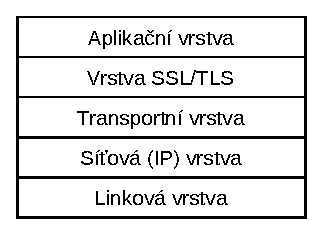
\includegraphics[width=0.3\textwidth]{fig/vrstvy-ssl}
  \caption{Vrstvy TCP/IP modelu s využitím SSL/TLS.}
 \label{fig:tls}
\end{figure}

Protokol TLS standardizuje IETF na základě původního protokolu SSL, který je
dnes již zastaralý~\cite{RFC7568}. Poslední verze protokolu TLS je
1.3~\cite{RFC8446}\footnote{Převyprávěná verze RFC 8446 je dostupná na \url{https://www.davidwong.fr/tls13/}}.

TLS vytváří obousměrný šifrovaný kanál mezi dvěma počítači, který zajišťuje:

\begin{itemize}

  \item Autentizaci: vždy se ověřuje identita serveru, identita klienta může být
  také ověřená. Pro ověřování se používají certifikáty X.509, které mohou být
  podepsány certifikační autoritou.

  \item Důvěrnost (utajení): po navázání spojení je obsah přenášené komunikace
  známý pouze komunikujícím stranám. Délka zpráv může být pozorovateli
  komunikace známá, TLS podporuje vycpávkový provoz.

  \item Integritu: Obsah zprávy není možné bez odhalení při přenosu upravit.

\end{itemize}

Samotný protokol TLS se skládá ze dvou podprotokolů:

\begin{itemize}

  \item \emph{Handshake protocol} se používá při navazování spojení a zajišťuje
  autentizaci komunikujících stran, domluvu kryptografických parametrů a
  sdílených klíčů.

  \item \emph{Record protocol} přenáší data mezi komunikujícími stranami.

\end{itemize}

\subsection{Certifikační autority}


Certifikační autorita (CA)\footnote{Text popisující CA je převzatý z~{\tt https://cs.wikipedia.org/wiki/Certifika\%C4\%8Dn\%C3\%AD\_autorita}.} je v asymetrické kryptografii subjekt, který vydává
digitální certifikáty (elektronicky podepsané veřejné šifrovací klíče), čímž
usnadňuje využívání Public Key Infrastructure (PKI) tak, že svojí autoritou
potvrzuje pravdivost údajů, které jsou ve volně dostupném veřejném klíči
uvedeny. Na základě principu přenosu důvěry tak můžeme důvěřovat
údajům uvedeným v digitálním certifikátu za předpokladu, že důvěřujeme samotné
certifikační autoritě.

Na Internetu působí mnoho komerčních certifikačních autorit, které obvykle mají
své veřejné klíče umístěny přímo ve webových prohlížečích a dalších programech,
čímž mohou uživateli zjednodušit rozhodování o míře důvěry webových serverů, ke
kterým se připojuje (ale též digitálně podepsaných e-mailů i jiných dat).
Existují též bezplatné certifikační autority nebo takové, které se řídí zákony
daného státu, vnitřními předpisy organizace a podobně.

Hodnota digitálního certifikátu je úměrná míře důvěry, kterou máme k údajům
v~něm uvedených. Proto je pro certifikační autoritu nejdůležitější důvěra, kterou
vůči svému okolí vzbuzuje (tj. že nevydá digitální certifikát s nepravdivými
údaji). Certifikační autorita proto musí adekvátním způsobem pečovat o svoji
důvěryhodnost, jinak by nebylo možné využít principu přenosu důvěry.

\subsection{Transparentnost certifikátů}

Aby bylo možné ověřit, že CA vydávají certifikáty poctivě, byl experimentálně
zaveden mechanismus transparentnosti certifikátů. Zapojené CA veřejně ohlašují
každý vystavený certifikát (případně precertifikát). Vydané certifikáty se
shromažďují v lozích (cerificate transparency log), kde je monitorovat nově
přidávané certifikáty a auditovat přítomnost certifikátu nalezených při
prohlížení webu.
